\section{Les Animaux Terrestres}
\subsection{Les chats c'est beau}
\lipsum[1]

\begin{figure}[htbp]
  \centering
  
\includegraphics[width=\textwidth]{paper/figures/chat1}
  \caption{Légende de l'image}
  \label{fig:chat1}
\end{figure}

\lipsum[2]

\begin{figure}[ht]
  \noindent
  \begin{minipage}{.6\textwidth}
    \lipsum[3]
  \end{minipage}
  \hfill
  \begin{minipage}{.35\textwidth}
    \centering
    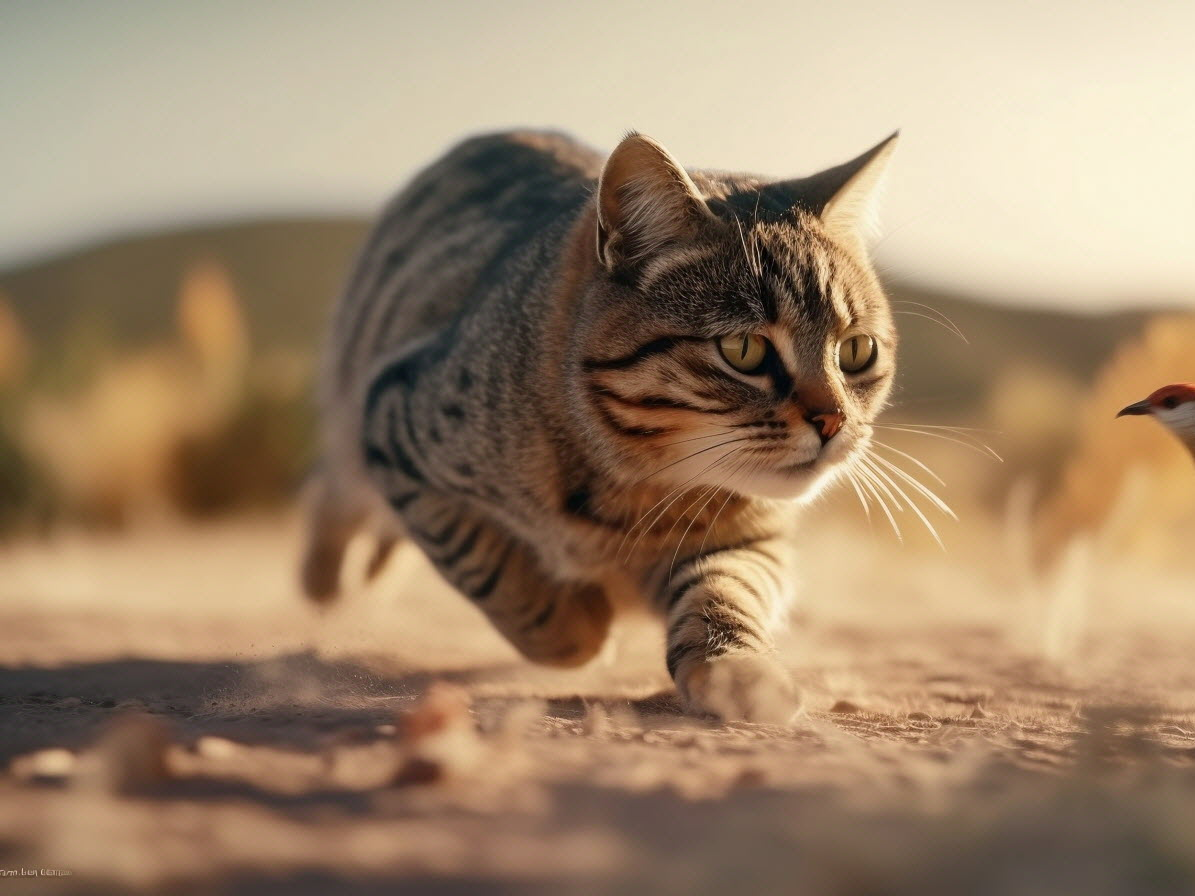
\includegraphics[width=6cm]{paper/figures/chat2}\\
    \caption{Chat volant}
    \label{fig:chat2}
  \end{minipage}
\end{figure}





\subsection{Les chiens boaf}
\lipsum[4-6]
\begin{figure}[htbp]
  \centering
  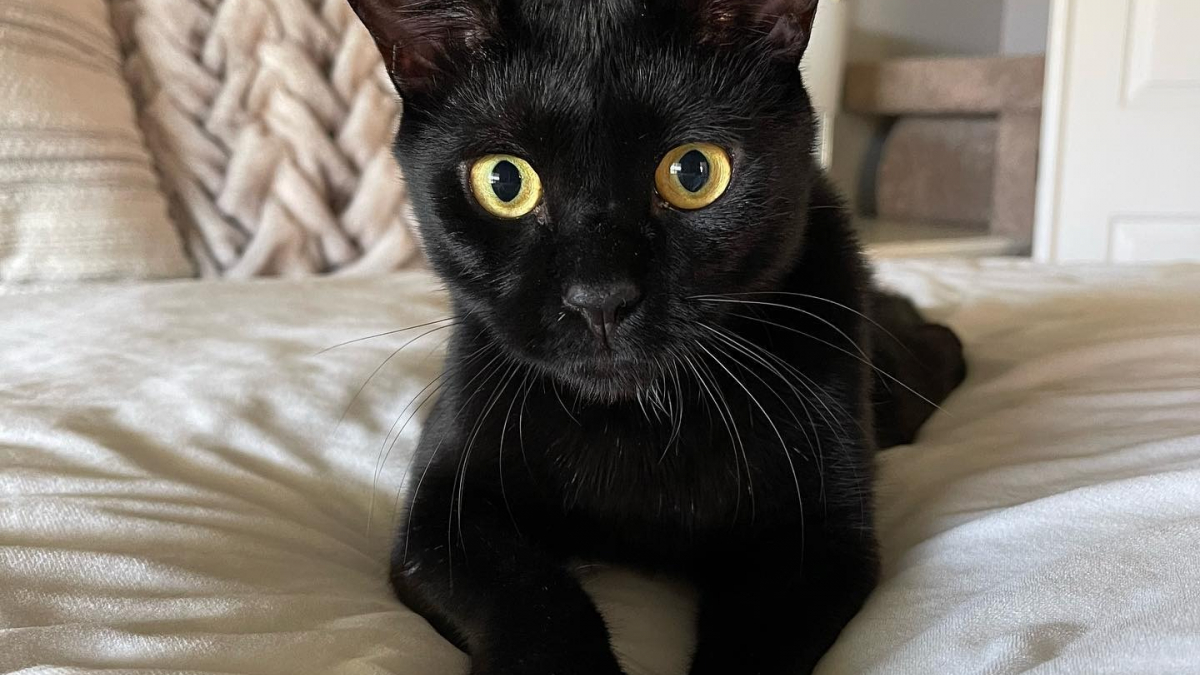
\includegraphics[width=\textwidth]{paper/figures/chat4.jpg}
  \caption{More Cats mais loin parce que latex (mettre un ! dvant le htbp pour forcer la position}
  \label{fig:chat4}
\end{figure}
\subsection{Les Wapiti c'est incroyable}
\lipsum[7-9]